%=============================================================================
% BACKGROUND
% What did other people do, and how is it relevant to what you want to do?

% ## Guidance

% -   Don’t give a laundry list of references.

% -   Tie everything you say to your problem.

% -   Present an argument.

% -   Think critically; weigh up the contribution of the background and
%     put it in context.

% -   **Don’t write a tutorial**; provide background and cite references
%     for further information.
%=============================================================================

\documentclass[../main.tex]{subfiles}
\graphicspath{{\subfix{../images/}}}

\begin{document}

This chapter shares the background of the dissertation by going deeper into the circumstances and motivations that led to the proposal of the project.

\section{Eating Habits in the UK}

This project was developed in Glasgow, UK and the Eatwell Guide is given by the Healthcare Service of England (NHS). To start with, it is important to learn about the lifestyle around food in the UK which is discussed in this section.

\subsection{Day Plan}

The average height and weight for men in England is 175.3cm and 83.6kg respectively, and for women it is 70.2kg and 161.6cm\cite{StatisticsRevealBritain2010}. This average person in the UK would aim to have three main meals a day.

\begin{figure}
    \centering
    \noindent\begin{subfigure}{.3\textwidth}
    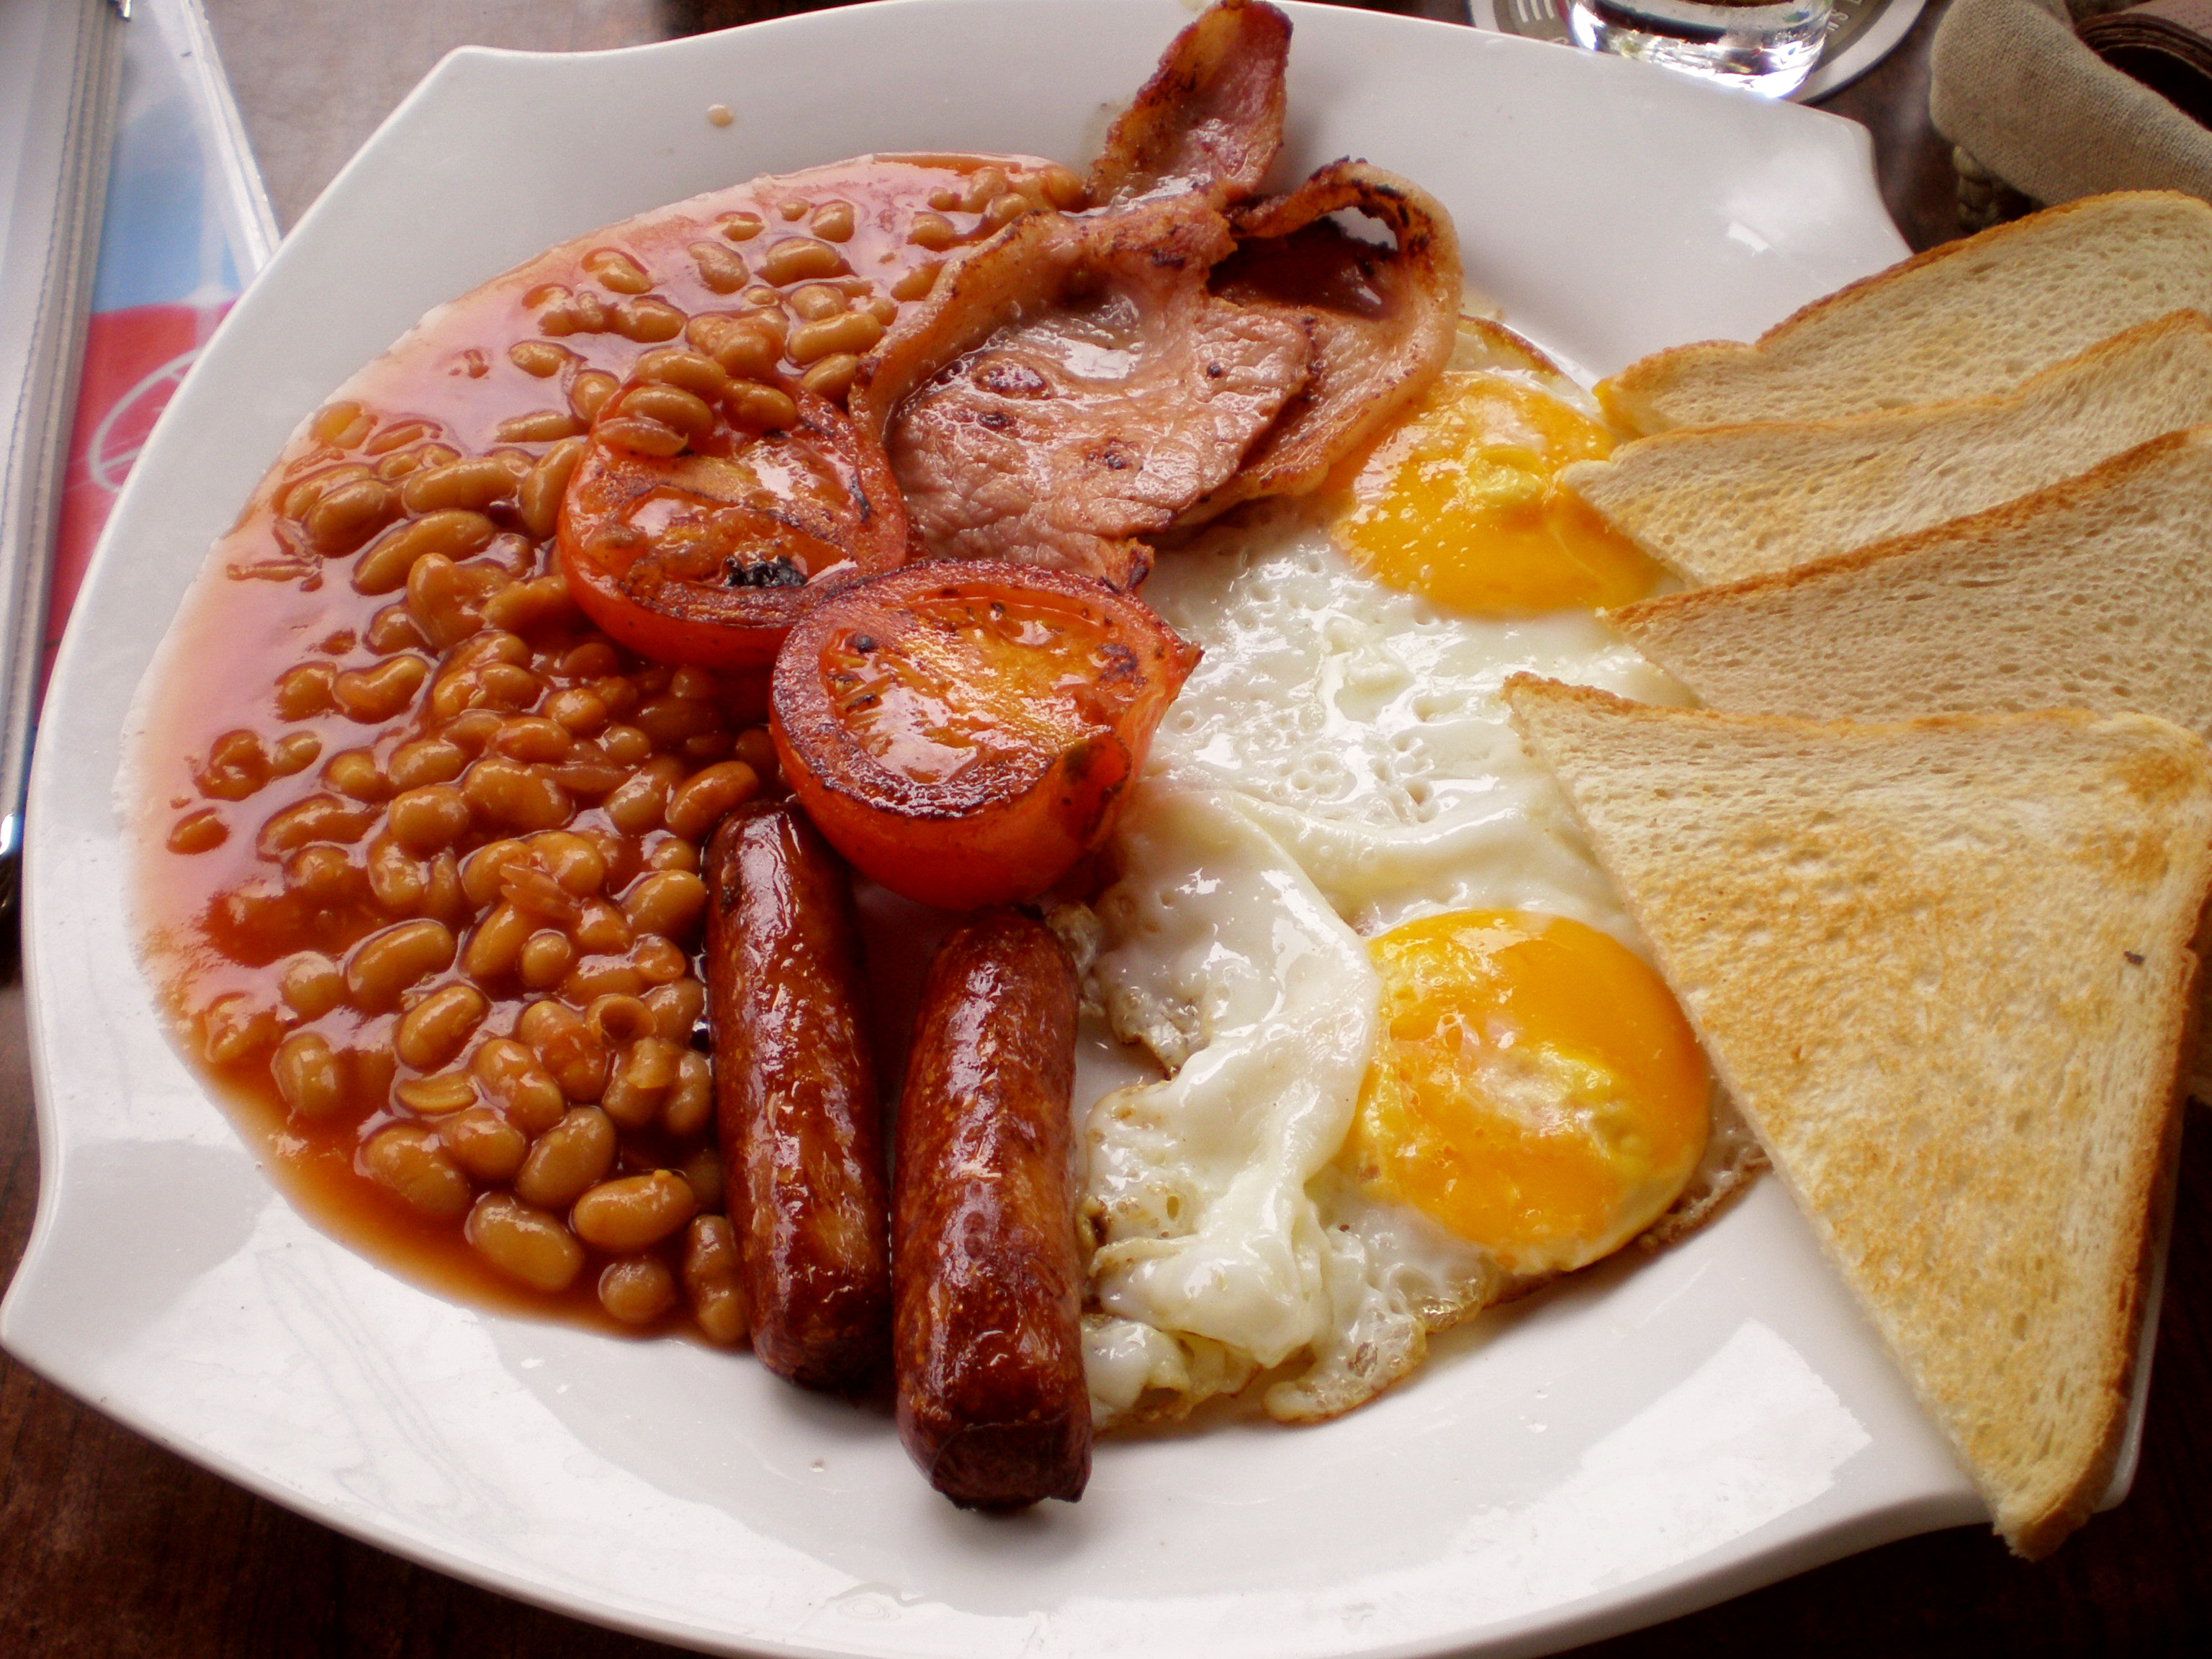
\includegraphics[width=\textwidth]{food/english_breakfast.jpg}
    \caption{English breakfast (\textit{from Freaky Fries on Wikimedia})}
    \end{subfigure}\hfill
    \begin{subfigure}{.3\textwidth}
    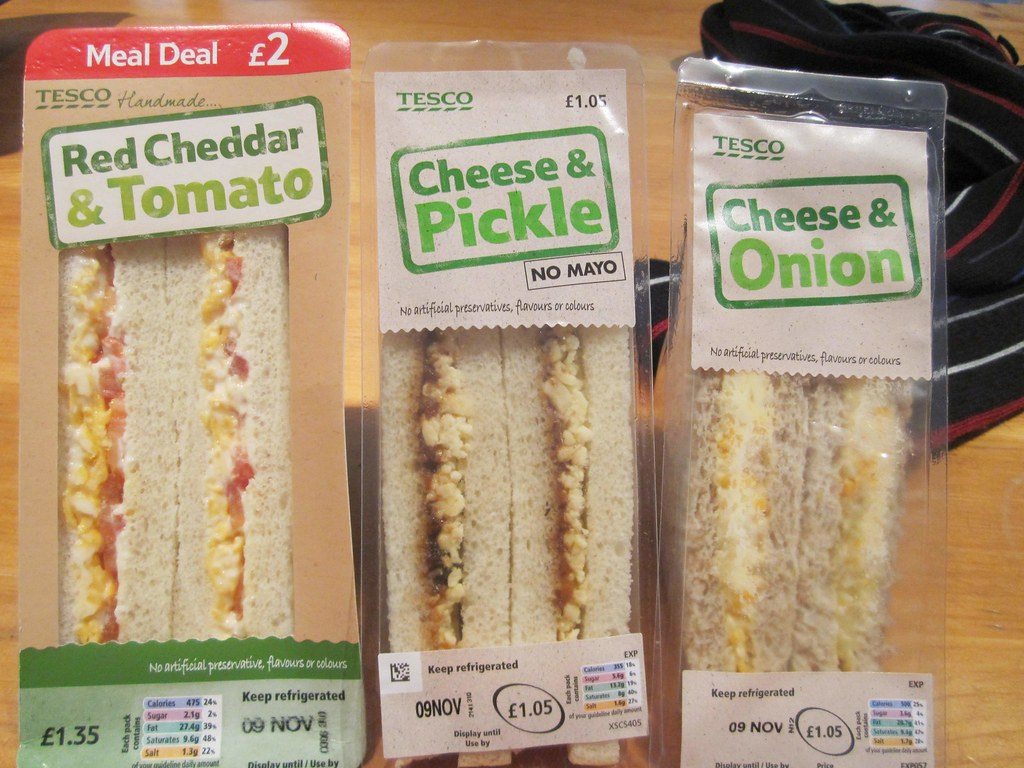
\includegraphics[width=\textwidth]{food/tesco_meal_deal.jpg}
    \caption{Tesco meal deals (\textit{from Rakka on Flickr})}
    \end{subfigure}\hfill
    \begin{subfigure}{.3\textwidth}
    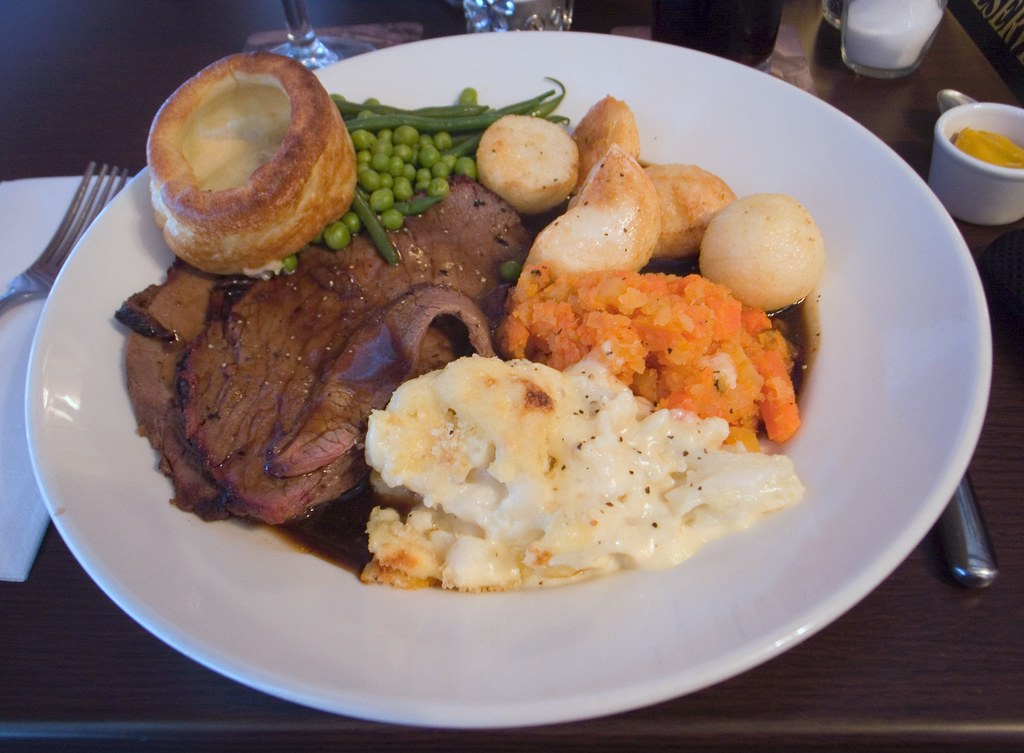
\includegraphics[width=\textwidth]{food/roast_dinner.jpg}
    \caption{Roast beef (\textit{from Adam Burt on Flickr})}
    \end{subfigure}
    \caption{Popular daily food consumed in the UK}
\end{figure}

\subsubsection{Breakfast}

The first meal of the day would be at any time for different persons, but popularly it is targeted to be between 07:00 and 09:00. Like an "American breakfast" is known to be a plate of pancakes, waffles, cereal, juice, bacon and egg, the "tranditional" "full English breakfast"\footnote{The quotes here are to indicate labels, as there may be those who have other beliefs.} consists of fried eggs, bacon, sausages, baked beans, black pudding and toast. It is a substantial meal that dates back to the 13th century \cite{HistoryTraditionalEnglish}. Given the pan-fried meat involved, some may deem it to be unhealthy, and a study suggests that skipping breakfast might be better than eating unhealthy foods \cite{pifferiCaloricRestrictionLongevity2019}. The NHS, however, suggests to start a day with a light bite, such as fruit or yoghurt, as the morning appetite will naturally increase and snacking will reduce \cite{HealthyBreakfastsPeople2018}.

\subsubsection{Lunch}

The second meal is expected to be midday (between 12:00 and 14:00), and in the UK, this meal is mostly simple and easy consisting of sandwiches (also known as "\textit{butty}") that can have many different items between the bread. The most common and cheap filling would be ham and cheese, or chips (therefore the popular "chip butty"), or just crushed crisps.

In the current times, the nation also feeds on meal deals (where normally a food and a drink could be bought at a discounted price) offered by chains like Greggs and Tesco.

\subsubsection{Dinner}

The "formal" meal -- Dinner, also called "\textit{Tea}" - is consumed between 18:00 and 20:00. In many cultures, it is supposed to be the largest meal of the day, but this may be discouraged as usually sleep follows dinner (therefore the consumed calories are not utilised). The rule followed for dinner is "meat and two veg" and typically that is a roast dinner. Since this meal is at the end of day when routine \& work has ended and temperature has fallen, one would also choose to unwind with a relatively "lavish", enjoyable meal. This could mean cooking cultural food, or simply do a takeaway from a nearby "\textit{chippy}" or stores.

\subsection{Processed Foods}

Over the years, there are options in the market that are easier and cheaper than cooking food yourself (previously discussed in \ref{sec:Motivation}). Processed foods are consumed daily by most people \cite{bbcShockingTransformationUK2021,HowBritsEating,rauberUltraprocessedFoodConsumption2020a}, and they are unavoidable as some processing may be essential, like milk \cite{EatingProcessedFoods2022}.

However, there are also frozen / microwave meals that can be prepared by heating for a few minutes in the microwave or oven, and can also be stored in the freezer for months. For example, pre-assembled pizzas are available in supermarkets, cost as much as a Greggs sausage roll (£1), and just requires baking in the oven for 10 minutes. However, a survey also discovered that one in ten people in the UK have not cooked a meal from scratch in over a year, choosing such alternatives for consumption \cite{alexanderOneTenPeople2019}. Food stores may also use taste enhancing chemicals (such as monosodium glutamate) to addict consumers to their strategically prices meals.

\begin{figure}
    \centering
    \noindent\begin{subfigure}{.3\textwidth}
    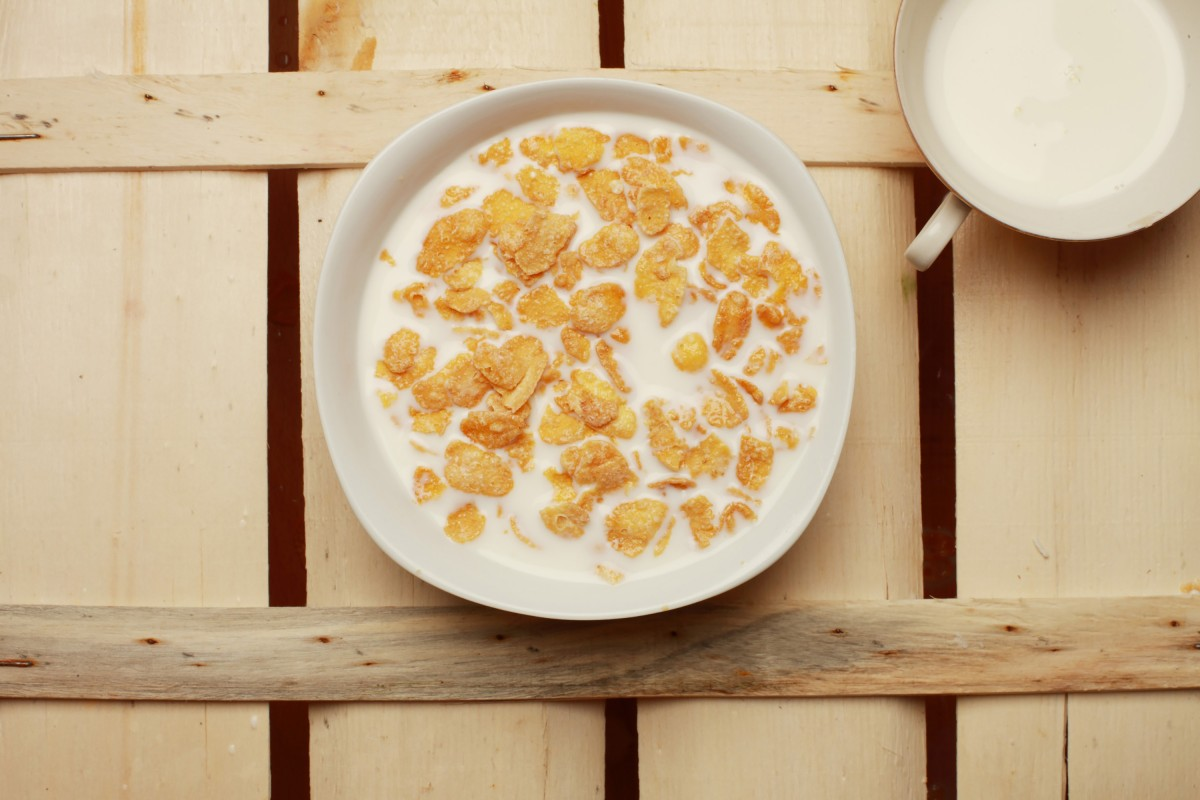
\includegraphics[width=\textwidth]{food/bowl_of_cereal.jpg}
    \caption{Bowl of cereal with milk (\textit{from PxHere})}
    \end{subfigure}\hfill
    \begin{subfigure}{.3\textwidth}
    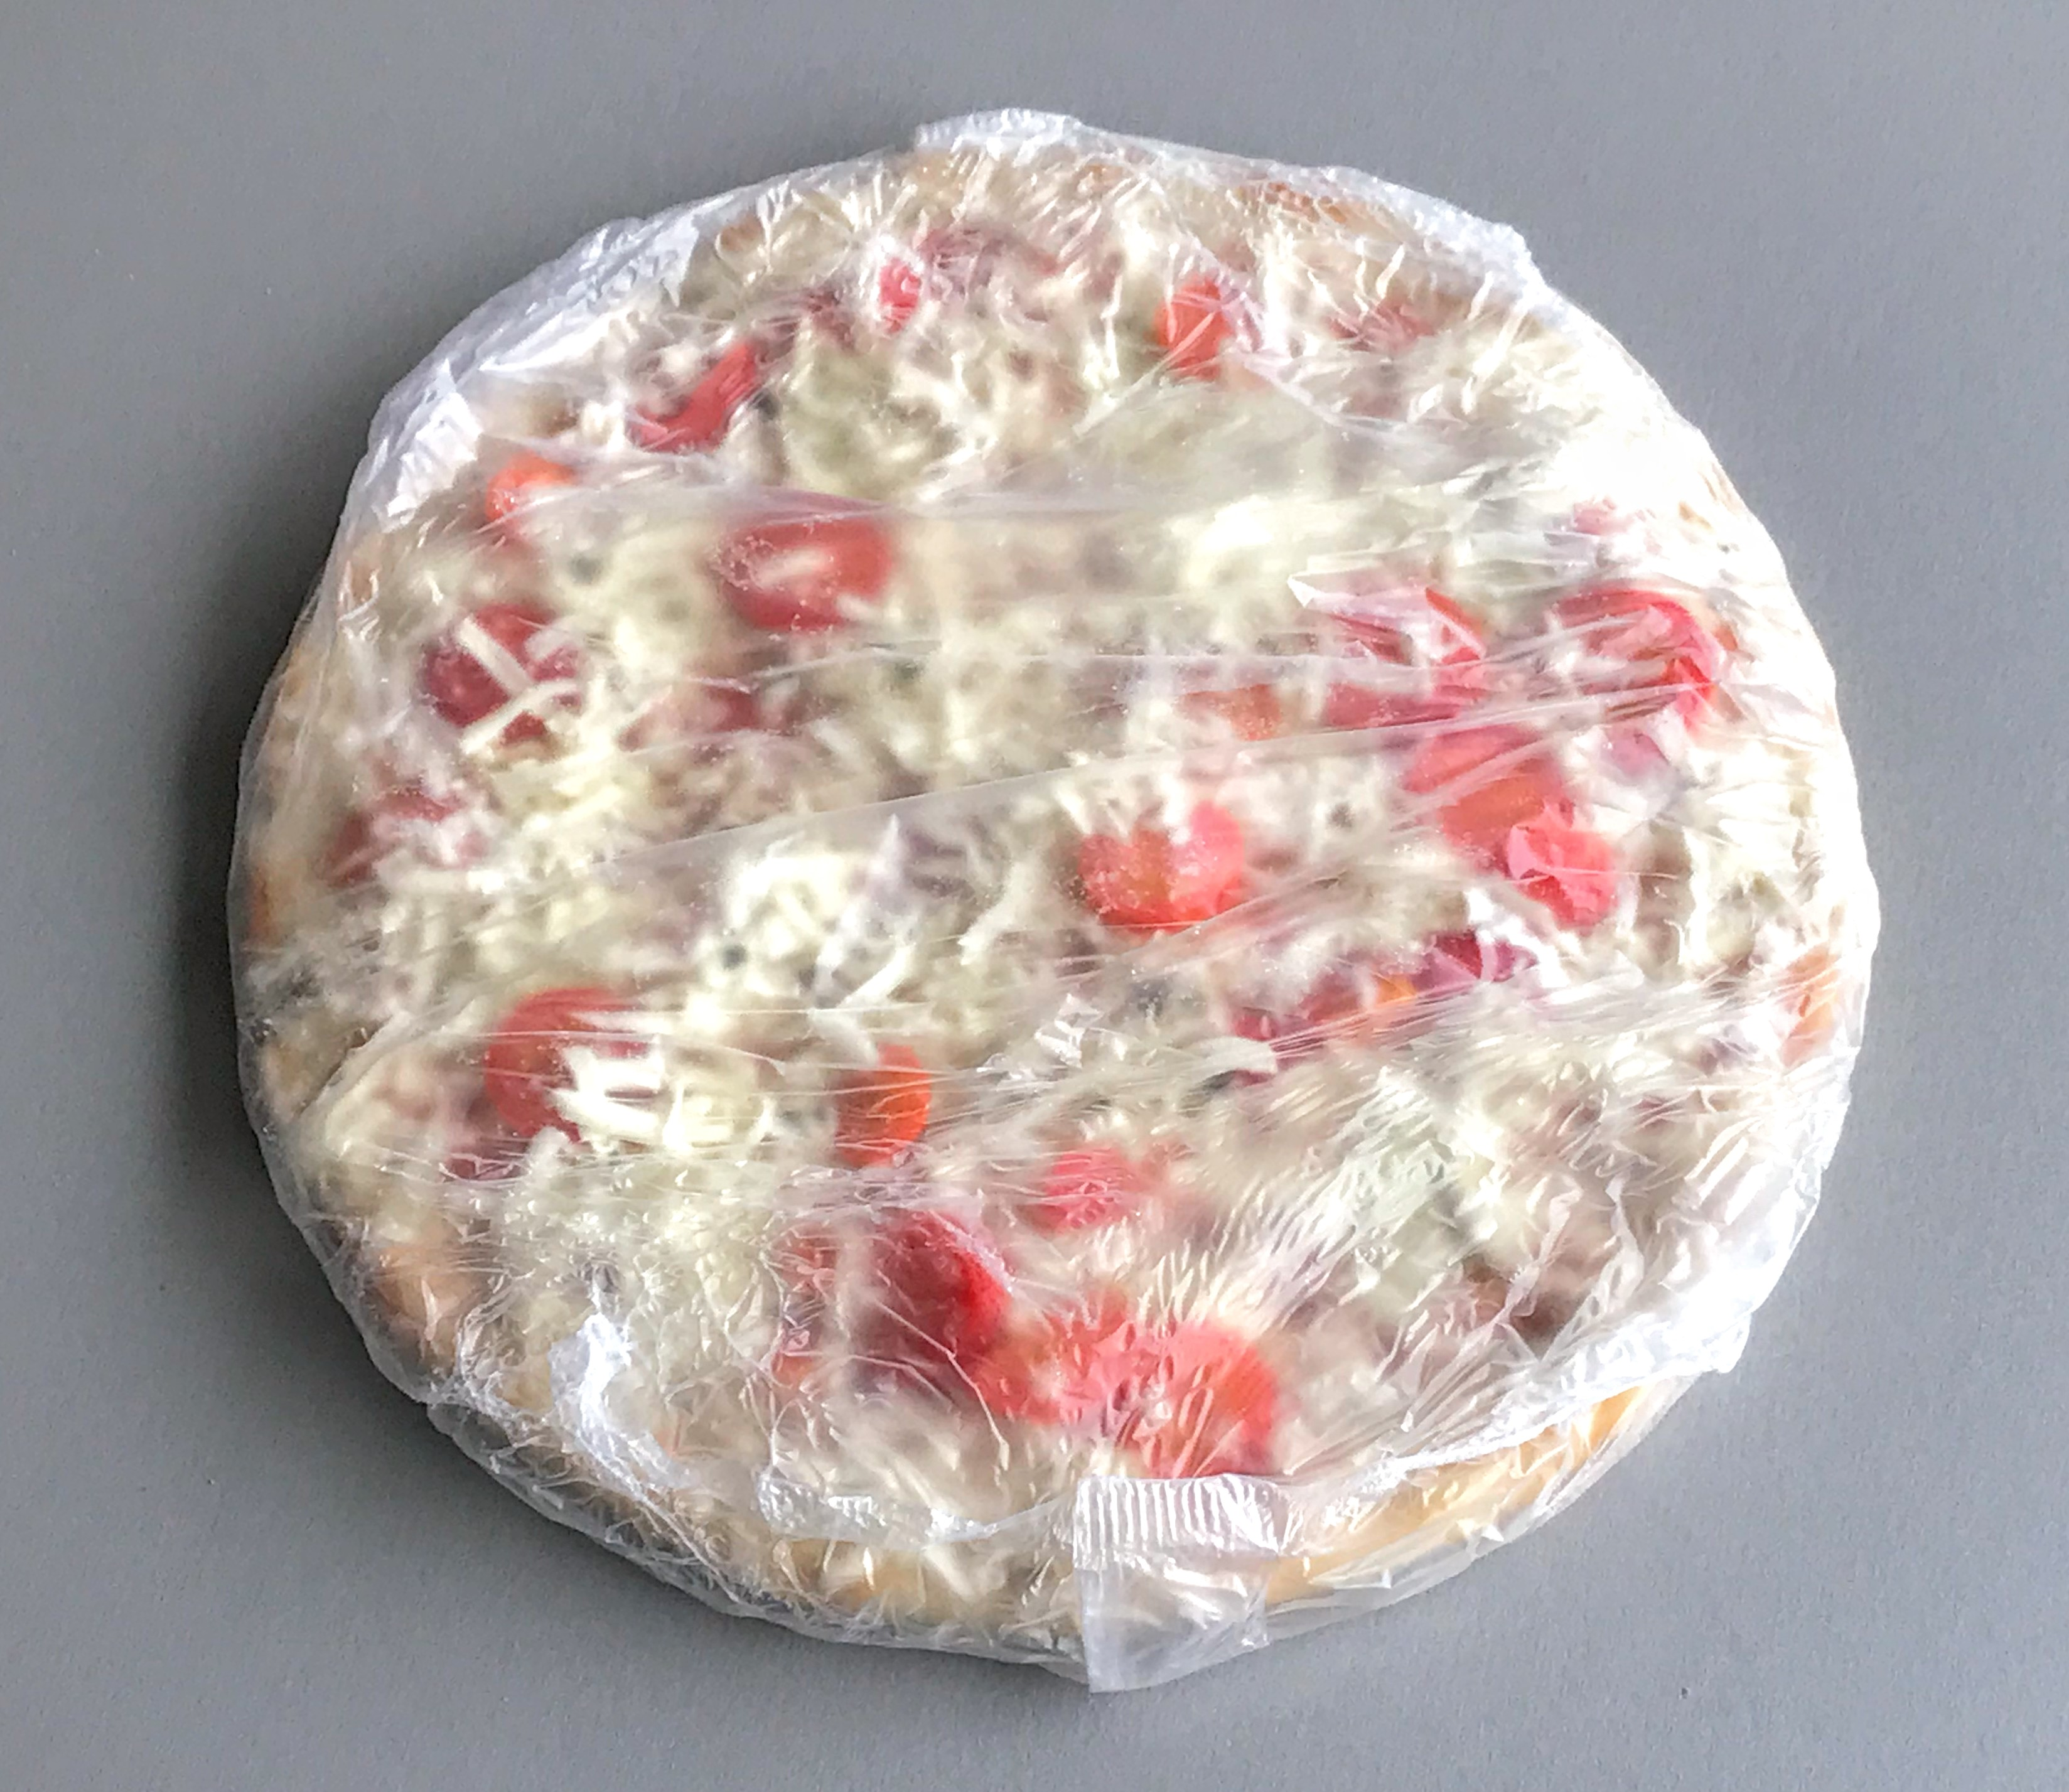
\includegraphics[width=\textwidth,trim={0 10cm 0 10cm},clip]{food/frozen_pizza.jpg}
    \caption{Frozen pizzas (\textit{from Amin on Wikimedia})}
    \end{subfigure}\hfill
    \begin{subfigure}{.3\textwidth}
    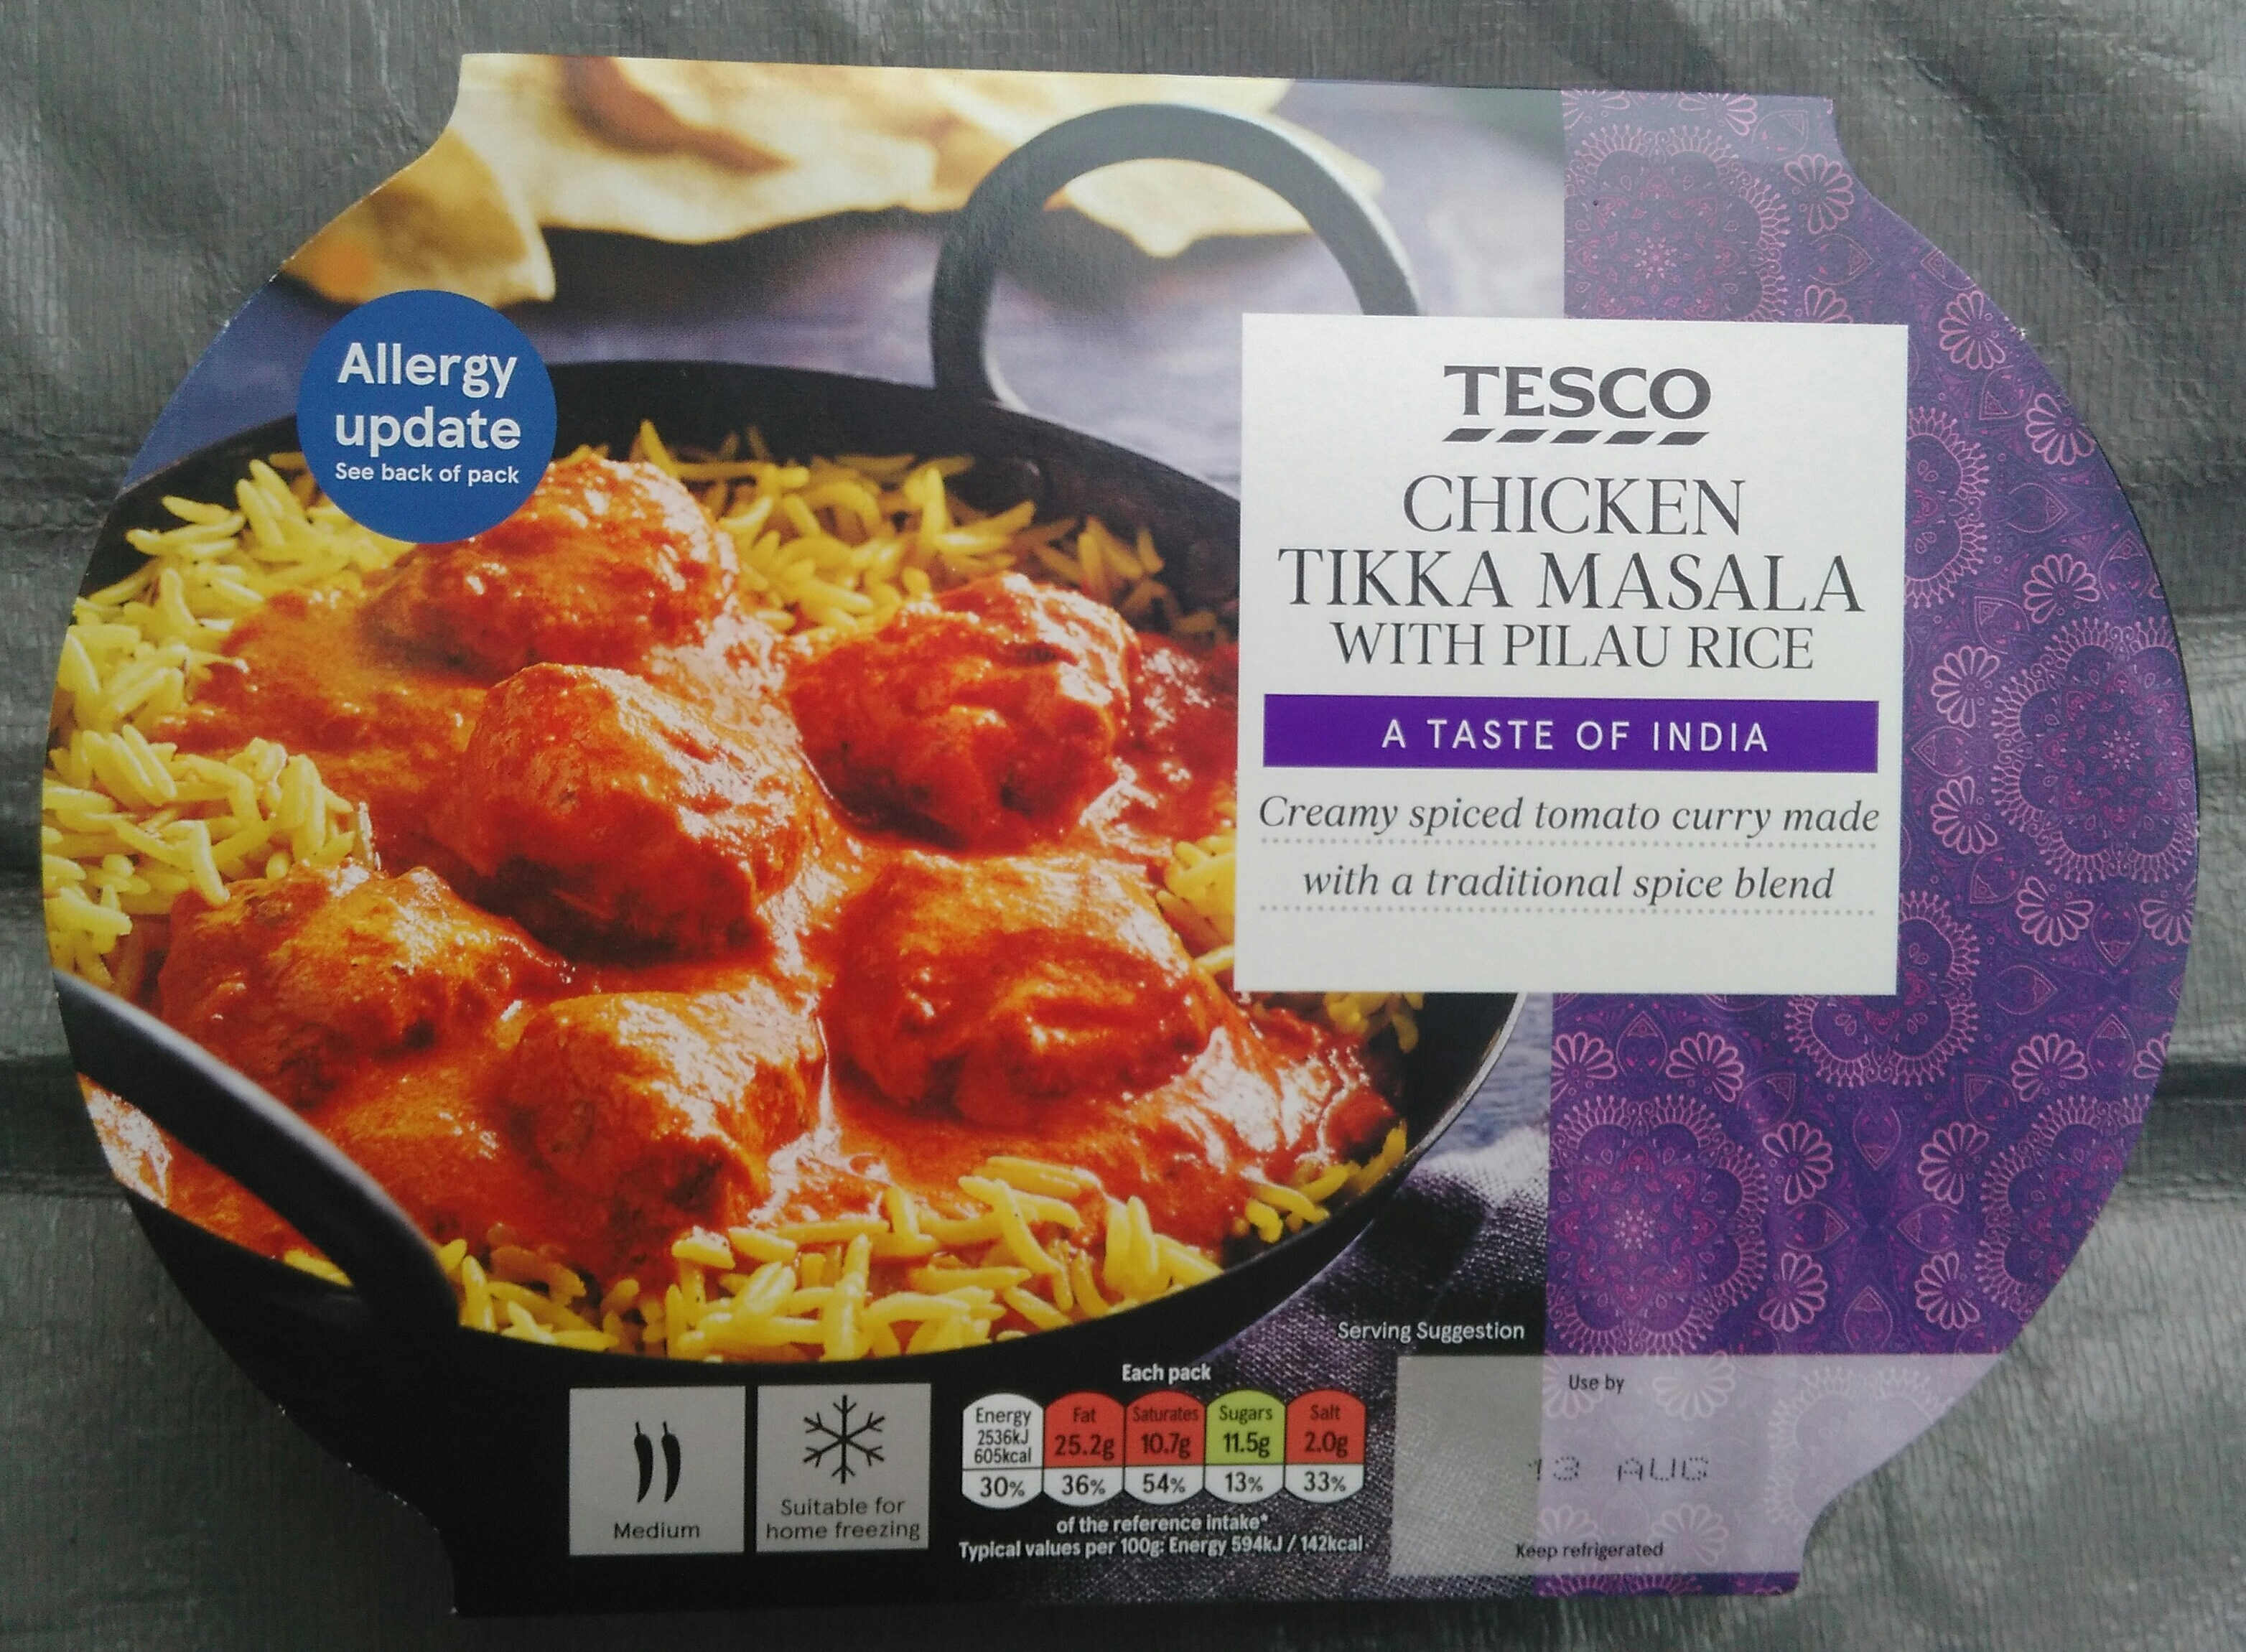
\includegraphics[width=\textwidth]{food/microwave_meal.jpg}
    \caption{Microwave meal (\textit{from Open Food Facts})}
    \end{subfigure}
    \caption{Examples of processed foods}
\end{figure}

\subsection{Various Diets}

While some cultures restrict meat, some view meat as a social celebration, a Reddit post discussed the consumption of meat in the UK \cite{WhoFeelsEvery2022} and most answers justify the meat for the protein and adding taste to relatively "boring" dinners that would otherwise consist of vegetables only. Through the day plan of a person in the UK (discussed in \ref{subsec:Day Plan}), a person could consume a lot of meat for all meals of the day (full breakfast that revolves around different meats, ham sandwich and roast chicken). Unfortunately, this causes a big impact on the environment since meat production creates a large percentage (60\%) of greenhouse gases every year \cite{milmanMeatAccountsNearly2021}.

A new trend has also been on the rise due to this called "veganism" where individuals would choose to cut out all animals product (such as dairy and poultry) from their diet. 3\% of the population in the UK are vegans \cite{DietaryChoicesBrits}. This has pushed research into finding meat alternative, and many companies to make inclusive meals, like a vegan sausage would use pea protein \cite{kassraieHowHealthyVegan}.

\begin{figure}
    \centering
    \noindent\begin{subfigure}{.55\textwidth}
    \includegraphics[width=\textwidth]{food/vegan_milk.jpg}
    \caption{Non dairy milk (\textit{from Veganbaking.net from USA on Wikimedia})}
    \end{subfigure}\hfill
    \begin{subfigure}{.42\textwidth}
    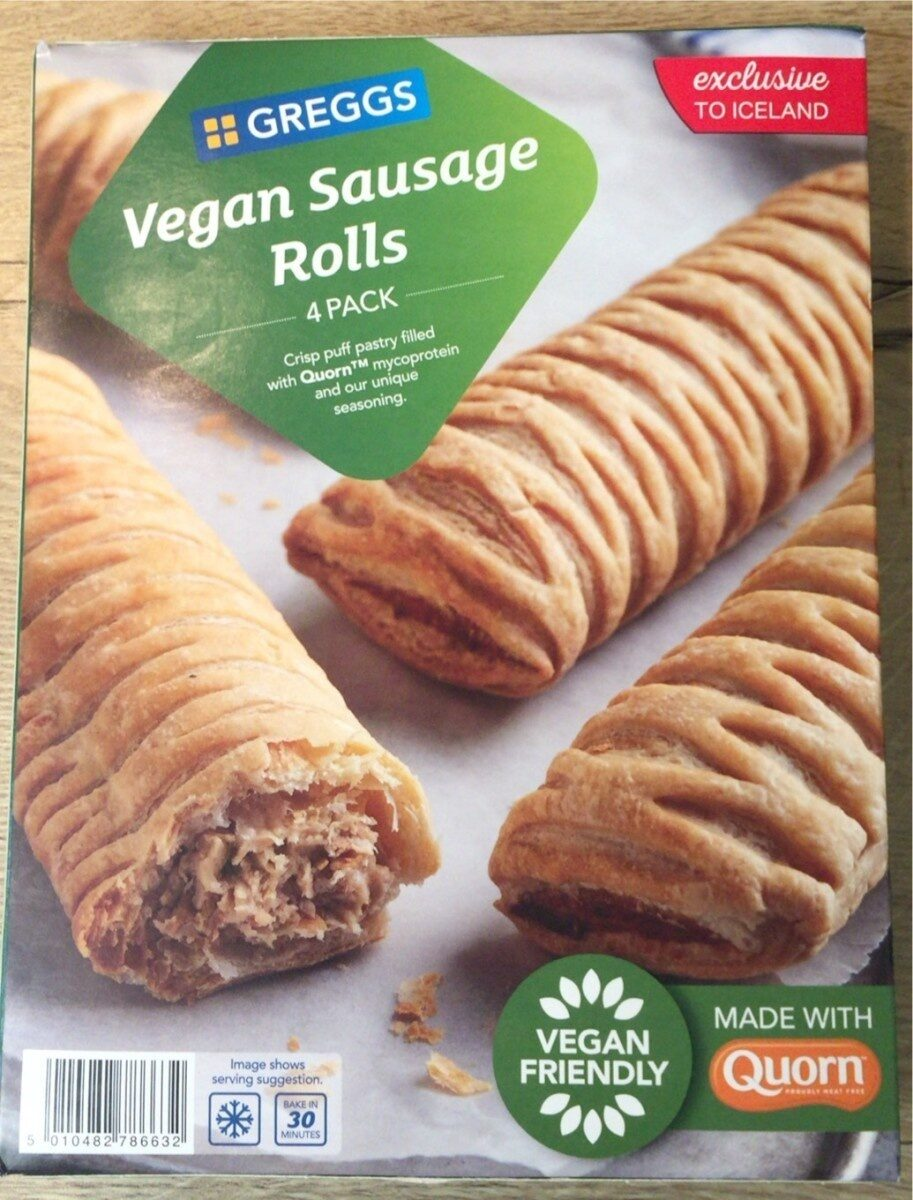
\includegraphics[width=\textwidth,trim={0 15cm 0 0},clip]{food/vegan_sausage_rolls.jpg}
    \caption{Vegan sauage rolls (\textit{from Open Food Facts})}
    \end{subfigure}
    \caption{Examples of vegan food}
\end{figure}

The student life cannot be ignored. Young\footnote{Mostly, but not necessarily.} adults and children, who require the health and nourishment to learn, often let their diets suffer as it is in relatively lower priority to deadlines. The main factor is time and energy to keep a diet. A day plan for a student may be cereal for breakfast, meal deal for lunch and microwave meal for dinner.

\section{Eatwell Guide}

The National Health Service (NHS) is a unified publicly funded healthcare system in the United Kingdom. Given the eating habits in the country discussed in \ref{sec:Eating Habits in the UK}, the NHS suggests a guide that encourages people to "eat well" by showing how many portions of each food group should be consumed for a healthy, balanced diet \cite{EatwellGuide, EatwellGuide2018}. The guide, previously called "the Eatwell Plate", includes instructions and food recommendations for the main essential food groups.

\foodgroup[Fruits]{Fruits \& Vegetables}

Being excellent sources of vitamins, minerals and fibre, at least 5 portions of fruits and vegetables \cite{DayWhatCounts2018} should be consumed everyday making up over a third of the food eaten in the whole day.

\foodgroup{Carbohydrates}

Starchy food (such as potatoes, bread, rice and pasta) should also make up a third of the food eaten similar to \ref{subsec:Fruits}. Meals can use this food group as the base - like pasta and meatballs, baked potatoes, sandwiches - therefore being the main source of nutrients and energy in one's diet. \cite{StarchyFoodsCarbohydrates2018}

\foodgroup{Dairy}

Some dairy (milk or alternatives) is important for calcium, keeping one's bones strong \cite{DairyAlternativesYour2018}. It should ideally make up about 10\% of daily intake, also avoiding products high in saturated fat.

\foodgroup{Protein}

As discussed in \ref{subsec:Various Diets}, consumption of meat is high in the UK, however there are alternatives such as beans, peas and lentils, that are low in fat. The NHS recommends to have at least two portions (each of 140g) of fish a week - one of which would be oily \cite{EatwellGuide2018}.

\foodgroup[Oils]{Oils \& Fats}

Only essential levels of fats should be taken, preferring unsaturated fats (such as vegetable oil instead of butter) as it helps reduce cholesterol in the blood.

\foodgroup{Fluids}

The instructions for 8 glasses of water a day is popular and should be followed everyday. Juices and smoothies also contribute to fluid consumption, but should be limited to 150ml a day. \cite{WaterDrinksYour2018}

\foodgroup{Sugars}

Foods high in sugar (like cakes \& chocolates) are not needed in the diet, but if included, should be in small amounts, since they have high calorie, and also affect parts of the body, such as teeth.

\section{Seeing a Professional}

The downside of the Eatwell Guide is that it is a general guide for everyone and hasn't been tailored for individuals - ones who may be of different age groups needing supplements, and therefore a professional can be approached to get a specific plan.

An expert who can provide guidance and prescriptions on eating habits is a \textbf{dietitian}. This may be confused with a nutritionist - the difference is that a dietitian is licensed and receive the title based on a classification by the World Health Organization \cite{whoClassification}. When seeking professional guide, there are likely to be follow ups, and accurate information is essential.

\section{The Client}

This project has been proposed by Dr. Oana M. Andrei - a lecturer at the University of Glasgow and the supervisor for this project - who has seen individuals logging their portion intake on paper, wishing to have a digital alternative. These logs are useful for dietitian visits (discussed in \ref{sec:Seeing a Professional}), but difficult to share on occasions.

\begin{figure}
    \centering
    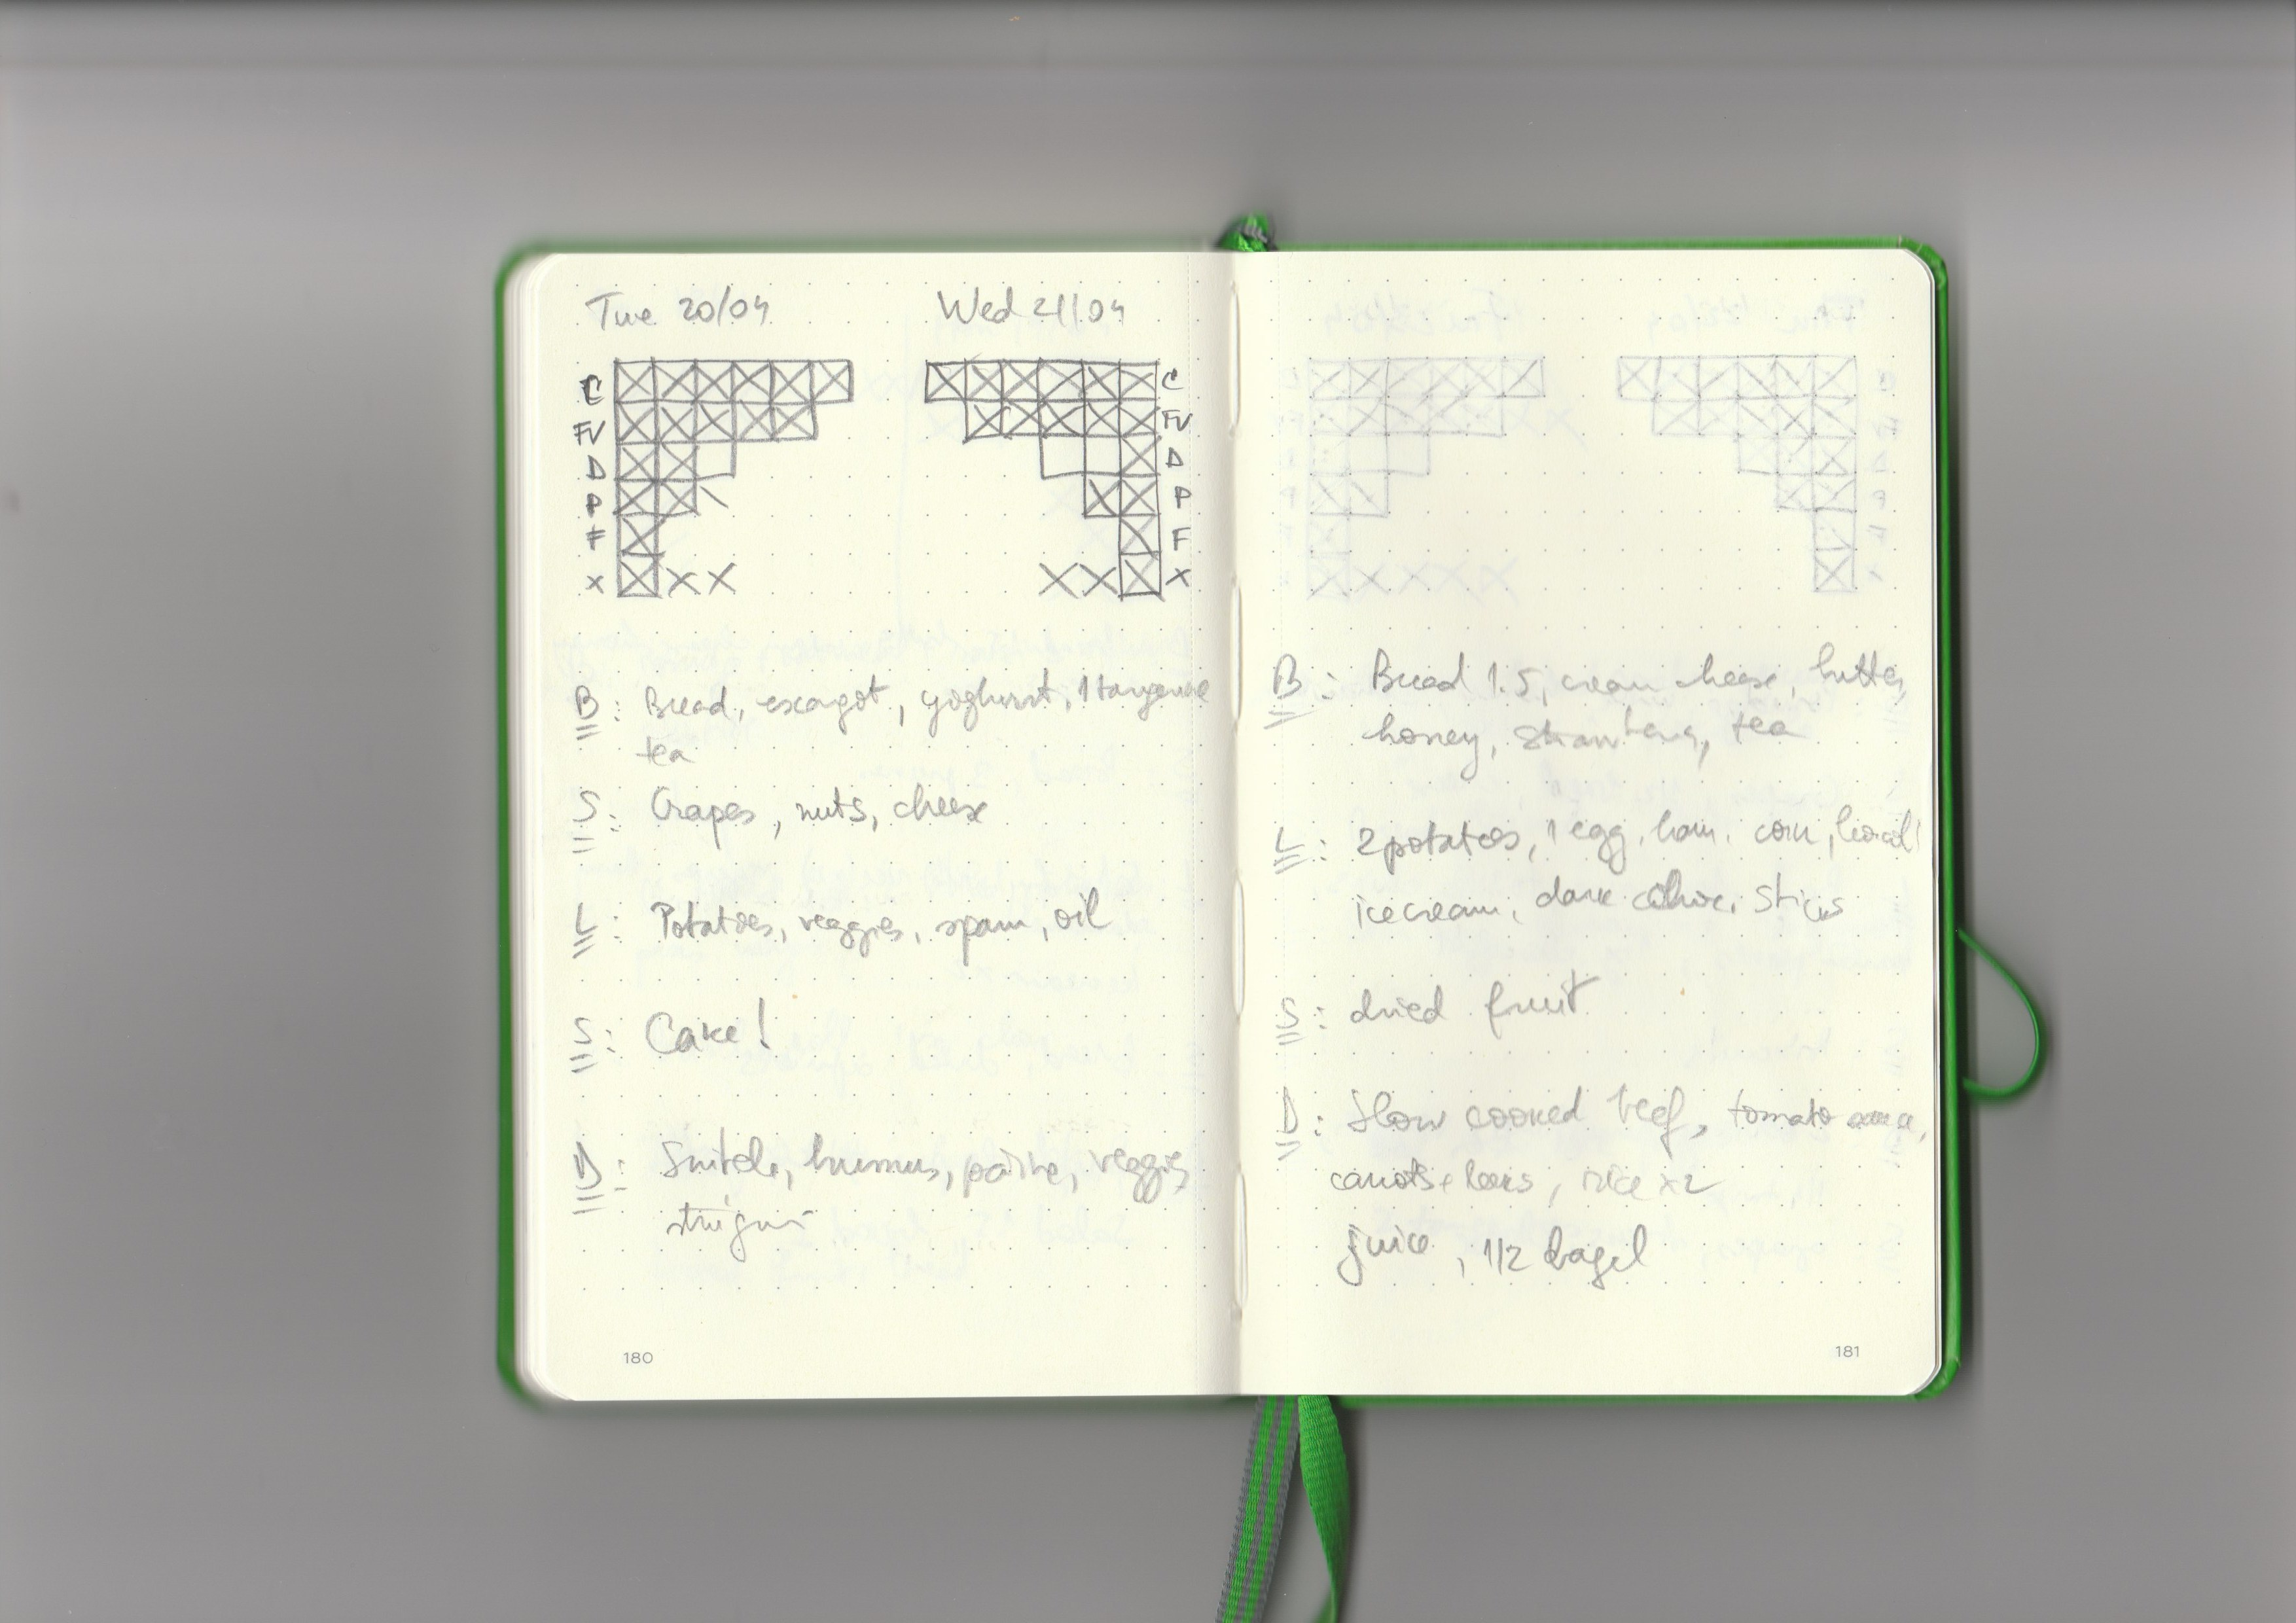
\includegraphics[width=\textwidth,trim={20cm 5cm 10cm 10cm},clip]{scans/portion2.jpg}
    \caption{A scan of an example paper log}%\label{fig:main_paper_log}
\end{figure}

From the example scan provided by Dr. Andrei (see \ref{fig:2.4}), a grid table can be seen with crosses (checkboxes) where each cell is supposed to be one portion. Therefore, in the first row, \code{C} (Carbohydrates) has 6 cells i.e. 6 portions. A full portion consumed is denoted by a cross, whereas half would be a slash. If consumption goes over the planned limit, the logs are added anyway (without the cells). In the lower half, there are notes and records maintained about what was eaten during the day as meals, like on Tuesday 20/04, for snacks (between breakfast and lunch) there were grapes, nuts and cheese, and on Wednesday 21/04, bread, cream cheese, butter, honey, strawberries and tea for breakfast. More scans are in the appendix (\ref{fig:A.2}) along with the initial example displayed at the first meeting (\ref{fig:A.1}), discussing the idea.

\section{Existing Apps}

Currently existing applications were briefly discussed and introduced in section \ref{sec:Motivation}. At the start of the project, there was a study conducted thinking why would one not use the competition instead \cite{wikiResearch}. This allowed research on features providing inspiration, downsides that would cause user frustration, and it was not limited to portion trackers.

\begin{figure}
    \centering
    \noindent\begin{subfigure}{.24\textwidth}
    \centering
    \frame{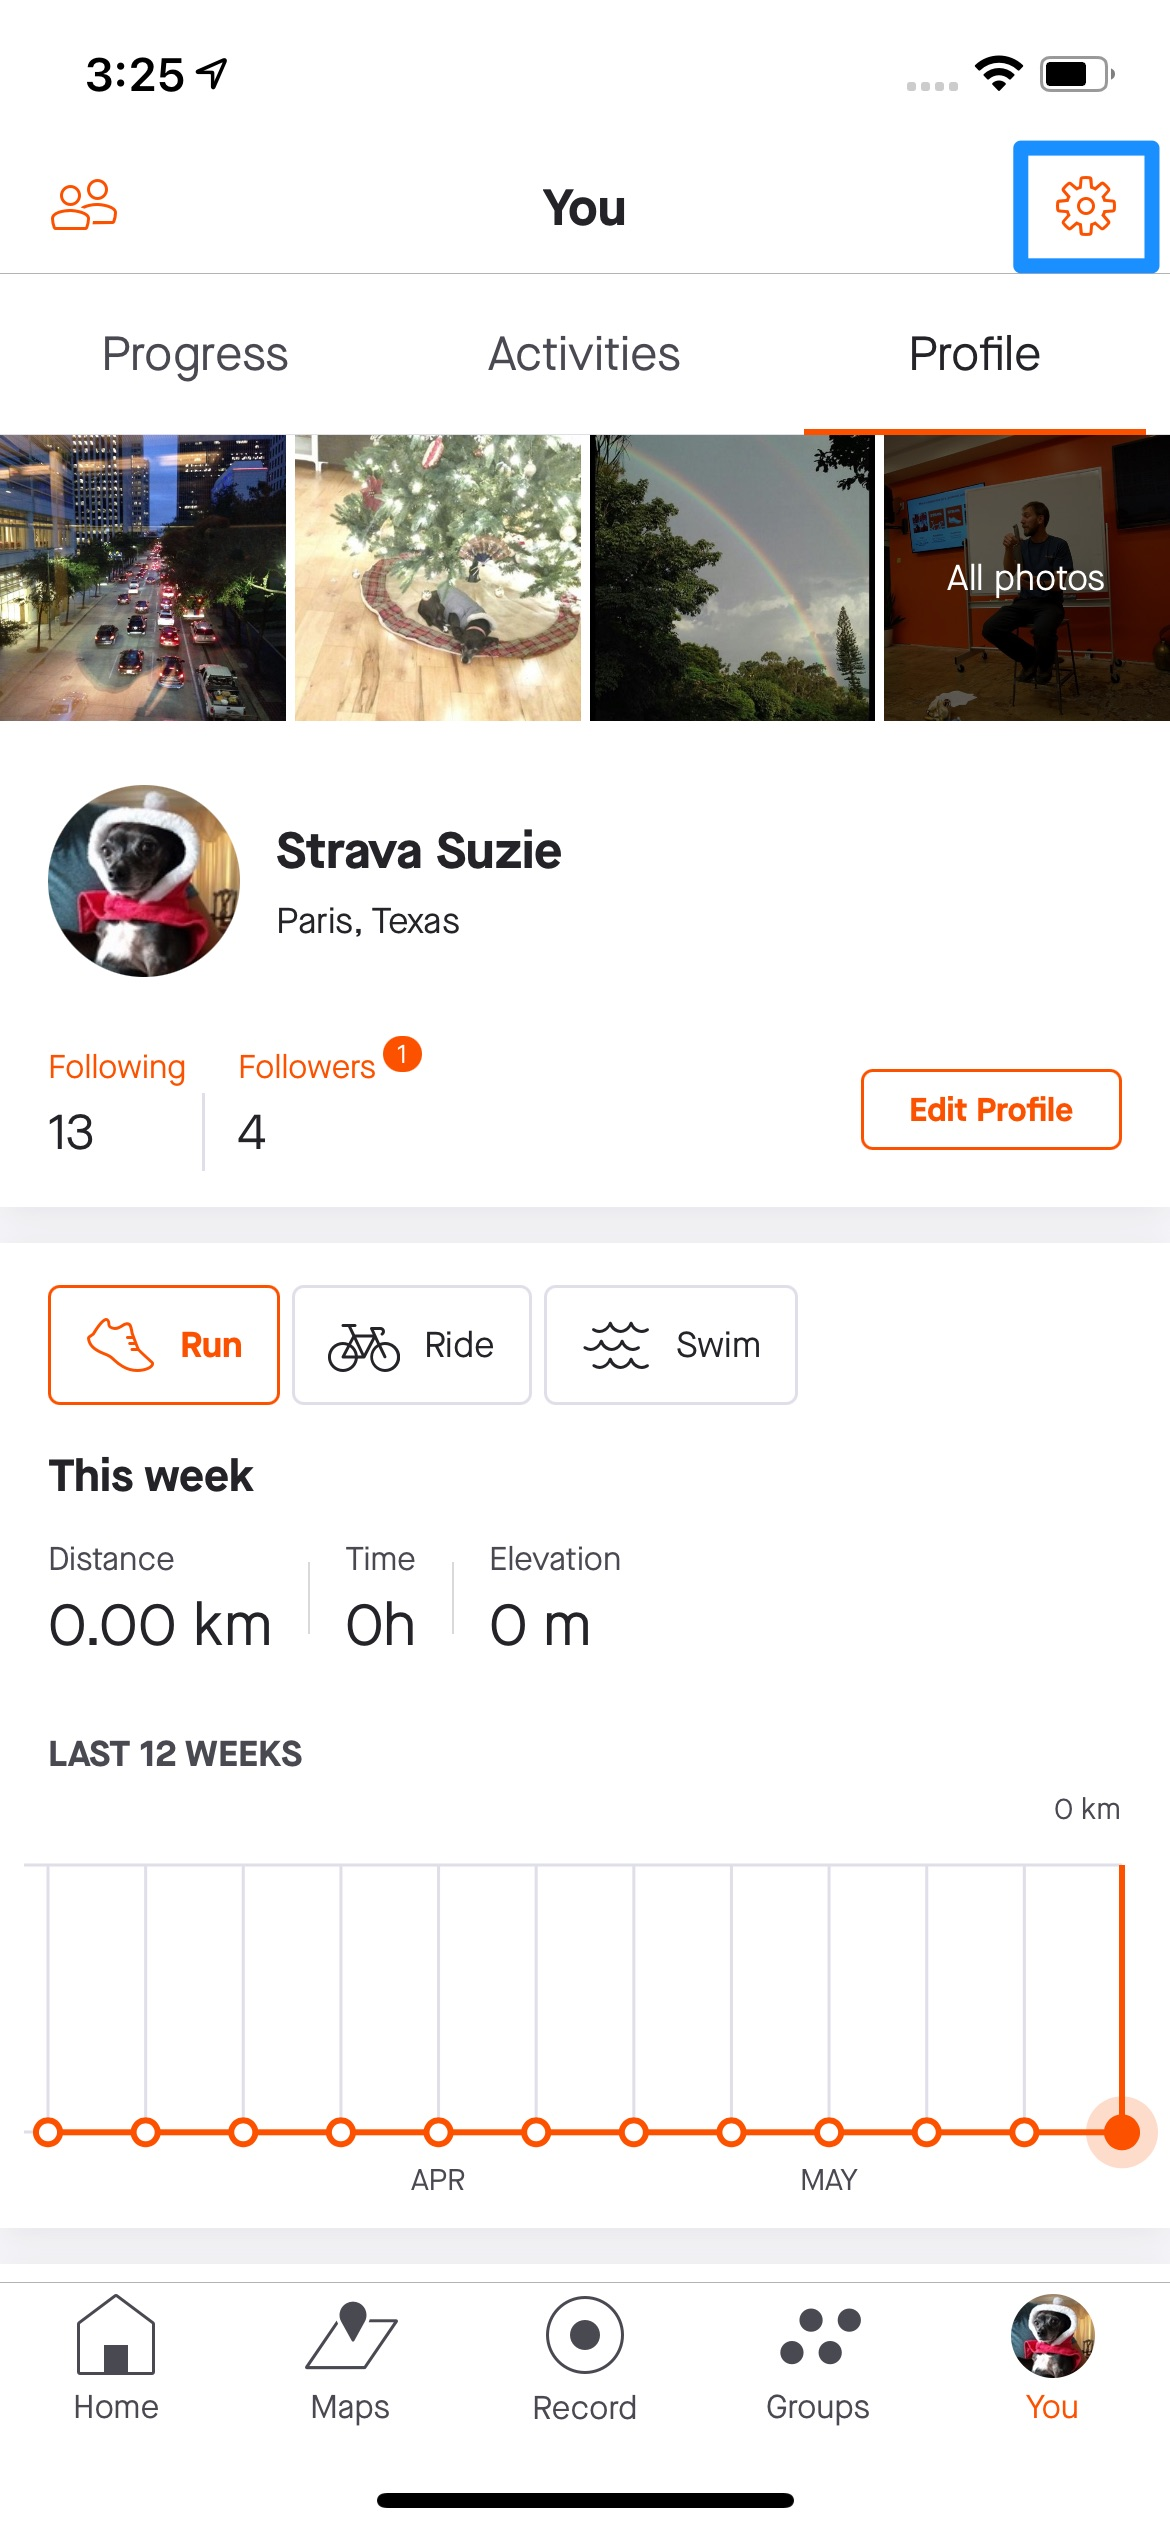
\includegraphics[height=5cm,trim={0 5cm 0 10cm},clip]{screenshots/strava_ss.jpg}}
    \caption{Strava}
    \end{subfigure}\hfill
    \begin{subfigure}{.24\textwidth}
    \centering
    \frame{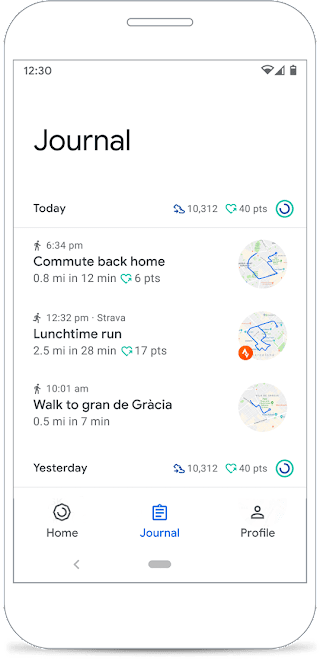
\includegraphics[height=5cm,trim={.5cm 4cm .5cm 2cm},clip]{screenshots/google_fit_ss.png}}
    \caption{Google Fit}
    \end{subfigure}\hfill
    \begin{subfigure}{.24\textwidth}
    \centering
    \frame{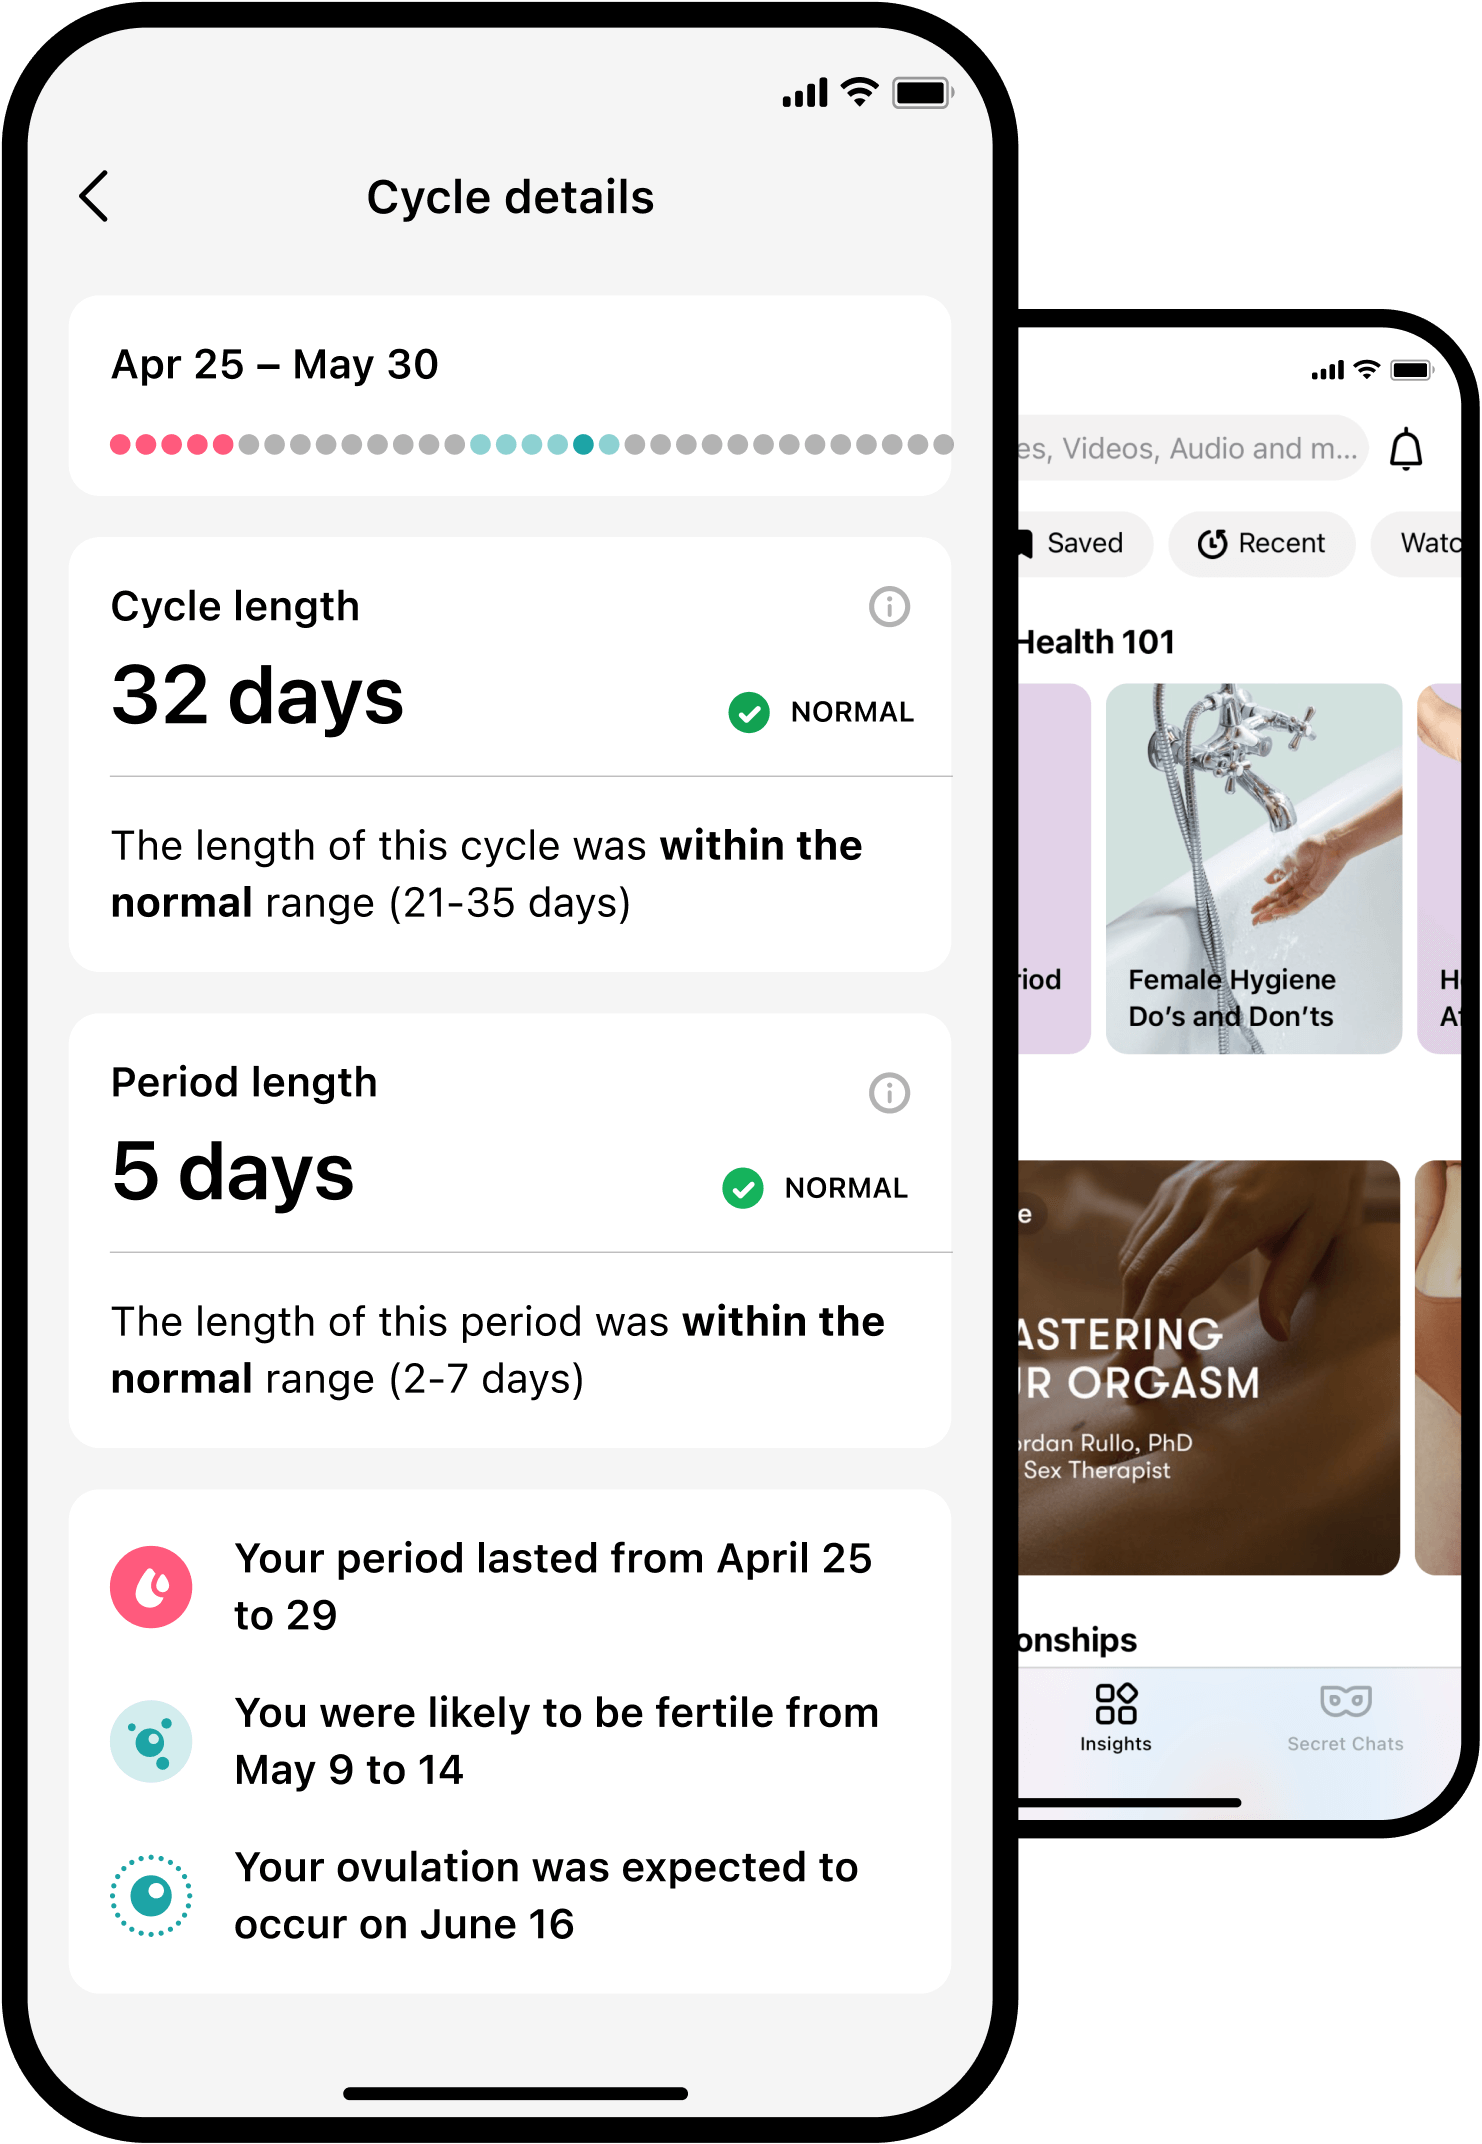
\includegraphics[height=5cm,trim={1cm 3cm 18cm 3.8cm},clip]{screenshots/flo_ss.png}}
    \caption{Flo}
    \end{subfigure}\hfill
    \begin{subfigure}{.24\textwidth}
    \centering
    \frame{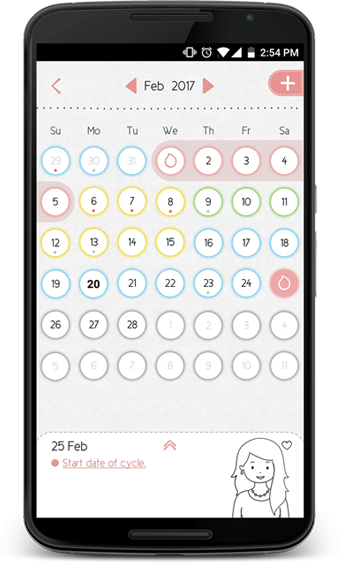
\includegraphics[height=5cm,trim={1.5cm 2cm 1.5cm 2.2cm},clip]{screenshots/maya_ss.png}}
    \caption{Maya}
    \end{subfigure}
    \caption{Preview of tracking applications}
\end{figure}

\subsection*{Fitness Trackers}

\textbf{\citetitle{StravaRunCycling}} records data for physical exercise activities (mostly cycling and running, that also use GPS data), incorporating social network features like sharing and liking ("\textit{kudos}") an activity. Activities in groups would also be automatically be displayed together when the system notices same place and time.

However, Strava also has an option to add activities manually - through importing from other device/services (like a Garmin), or just the statistic data you would know (like pace for a run), and during this, the form could also adjust for different sports. Strava does not log food intake.

\textbf{\citetitle{GoogleFit}} is Google's approach of a fitness tracker, released in 2014. It uses the simple, minimal Google interface design and layout which should be aimed for. The application provides its own means of logging and using sensors in a device, but it heavily focuses on providing APIs in order to be the general, overall application that would aggregate data from other device and services.

\subsection*{Period Trackers}

\textbf{\citetitle{FloOvulationCalendar}} released in 2015, focusing to track menstruation in women. It supports users through each stage of the cycle by notifying (push-notifications) them about predictions, and helping in any two approaches - tracking the cycle, or tracking fertility. This would be similar to what this project would aim for - providing notifications to remind users, and allowing users to track progress to lose/maintain weight, or increase for bulk/BMI.

\textbf{\citetitle{Maya}} also supports women by tracking cycles, but also by providing forums and resources. The application includes a calendar view that can display visualisations \& graphs.

\subsection*{Portion Trackers}

\textbf{\citetitle{FitbitAppDashboard}} is very popular for being the companion application for devices from the company, however it aims to provide a lot more functionality. There are resources, including videos, that can help users in fitness. More importantly, the application allows food tracking; the dashboard is highly customisable so the option can be removed if required. However, the tracking allows items to be added easily by scanning any QR codes that a packaged food would have.

\textbf{\citetitle{BaritasticHome}} specialises in the branch of medicine that deals with the causes, prevention and treatment of obesity ("\textit{bariatric}") and therefore the application is tailored for patients of the same. The interface provides a graph with card view, along with an appropriately sized action button in the bottom-middle that can allow certain tasks. It includes reminders and journal logging.

\textbf{\citetitle{PortionMonitorApps}} from Tiny apps appears to be a very simple, basic and possibly outdated (last updated October 2019), but the dashboard includes a main table where the logging can occur. The rows/x-axis of the table are food groups (carbohydrates, protein) and columns/y-axis are the meals (breakfast, snack1, lunch). It can also display graphs for a time period.

\textbf{\citetitle{LifesumHealthApp}} is a paid application that specialises in food track with a range of fancy functionalities such as a food database, barcode scanner, and meal ratings. An interesting feature here is the list of recipes the application can provide that are in compliance with the diet plan.

\section*{Summary}

Food has many aspects and backgrounds. In the UK itself, there is history and variety to meals available to people, ranging from all vegan diet to a high meat consumption. Some of it would include food that may be unhealthy for regular consumption as they include ingredients that should be taken in moderation, and therefore the National Health Service (NHS) provide instructions through the Eatwell Guide that layouts the essential food groups and the appropriate amount for a healthy, balanced diet. In specific cases where one may require professional help, dietitians are helping people to have healthier diets by prescribing diets tailored to individuals. Those who wish to aid this, log their intake may be doing it on paper, or other applications such as Google Fit, Fitbit or Lifesum, that vary a lot in features. These differences and features were studied, and along with the motion of promoting healthier diets, an overall application, that \textit{checks all boxes} and tailors to this purpose by helping and motivating users, would be inspired.

\end{document}
